\documentclass[12pt,a4paper]{article}

% To use this template make changes to following:
% 1. Fill-ables section.
% 2. Instructions.
% 3. Marks table.
% 4. Actual questions.

% ================================ 1. Fill-ables ================================
\newcommand\University{National University of Computer and Emerging Sciences}
\newcommand\Department{School of Engineering}
\newcommand\Campus{Islamabad Campus}
\newcommand\Semester{Spring 2015}
\newcommand\Exam{Sessional--II}
\newcommand\Subject{CS210--Data Structures and Algorithms}
\newcommand\ExamDate{Monday, April 27, 2015}
\newcommand\InstructorOne{Attique Dawood}
\newcommand\InstructorTwo{\null~}
\newcommand\InstructorThree{\null}
\newcommand\TotalTime{01 Hours}
\newcommand\TotalMarks{50}
\newcommand\TotalQuestions{5}
\newcommand\TotalPages{\pageref{LastPage}} % Automatic: No need to change this.
% Marks of each question
\def\Qone{10}
\def\Qtwo{10}
\def\Qthree{10}
\def\Qfour{10}
\def\Qfive{10}
\def\Qsix{0}
\def\Qseven{0}
\def\Qeight{0}
\def\Qnine{0}
\def\Qten{0}
% ============================================================================

% ============== 2. Packages ==============
\usepackage{amsmath}
\usepackage{float}
\usepackage{graphicx}
\usepackage[hyphens]{url}
\usepackage[hidelinks]{hyperref}	% Clickable links to figures, references and urls.
\usepackage{lastpage}
\usepackage{array}
\usepackage{fancyhdr}
% Drawing packages.
\usepackage{pgf}
\usepackage{tikz}
% Listings for formatting code.
\usepackage{listings}
\usepackage{textcomp}

% General listings options.
\lstset{breaklines=true, basicstyle=\footnotesize\ttfamily, tabsize=4, numbers=left, stepnumber=1, frame=none, showstringspaces=false, upquote=true}
% C++ specific high-lighting. Comments are 50/50 shades of green/black and strings coloured with 60/40 red/black mixture.
\lstset{language=[ISO]C++, commentstyle=\color{green!50!black}, keywordstyle=\color{blue}, stringstyle=\color{red!60!black}}

% Table cell alignment directives.
\newcolumntype{L}[1]{>{\raggedright\let\newline\\\arraybackslash\hspace{0pt}}m{#1}}
\newcolumntype{C}[1]{>{\centering\let\newline\\\arraybackslash\hspace{0pt}}m{#1}}
\newcolumntype{R}[1]{>{\raggedleft\let\newline\\\arraybackslash\hspace{0pt}}m{#1}}

% Line spacing.
\def\SingleSpacing{\def\baselinestretch{1}\large\normalsize}
\def\DoubleSpacing{\def\baselinestretch{1.5}\large\normalsize}

% Margins.
\setlength{\oddsidemargin}{0in}
\setlength{\evensidemargin}{0in}
\setlength{\headheight}{28pt}
\setlength{\headsep}{2.5pt}
\setlength{\topmargin}{-55pt}
\setlength{\textwidth}{6.5in}
\setlength{\textheight}{10.75in} % Actual: 10.75in

% ============================= 3. Header and Footer ============================
\pagestyle{empty}
% Header
\chead
{
	{\large\textbf{\University}}\\
	\begin{minipage}{0.45\textwidth}
	\begin{center}
	{\small\textbf{\Department}}
	\end{center}
	\end{minipage}
	\begin{minipage}{0.45\textwidth}
	\begin{center}
	{\small\textbf{\Campus}}
	\end{center}
	\end{minipage}
}
% Footer
\lfoot{{\small\Exam}}
\cfoot{{\small\Semester}}
\rfoot{{\small Page \textbf{\thepage}~of \textbf{\TotalPages}}}
\renewcommand{\headrulewidth}{0.4pt}
\renewcommand{\footrulewidth}{0.4pt}
% ================================= 4. Front Page ===============================
\begin{document}
% A cute macro to add up marks of all individual questions. Uncomment if you want to use this.
\pgfmathtruncatemacro\TotalMarks{\Qone+\Qtwo+\Qthree+\Qfour+\Qfive+\Qsix+\Qseven+\Qeight+\Qnine+\Qten}
% Use this macro if marks are in decimal points
%\newcommand\TotalMarks{\pgfmathsetmacro\TotalMarks{\Qone+\Qtwo+\Qthree+\Qfour+\Qfive+\Qsix+\Qseven+\Qeight+\Qnine+\Qten}}
\begin{minipage}[t]{0.6\textwidth}
\begin{flushleft}
\DoubleSpacing
{\Large\textbf{\Subject}}\\
{\normalsize\ExamDate}\\
{\large\textbf{Course Instructor}}\\
{\normalsize\InstructorOne}\\
{\normalsize\InstructorTwo}\\
{\normalsize\InstructorThree}
\end{flushleft}
\end{minipage}
\begin{minipage}[t]{0.01\textwidth}
~
\end{minipage}
\begin{minipage}[t]{0.325\textwidth}
\DoubleSpacing
{\normalsize Serial No:}\\
{\Large\textbf{\Exam}}\\
{\large\textbf{Total Time: \TotalTime}}\\
{\large\textbf{Total Marks: \TotalMarks}}\\[1cm]
\rule{5cm}{0.2mm}\\[-0.25cm]
{\small Signature of Invigilator}
\end{minipage}
\SingleSpacing
~\\[1.5cm] % Extra space.
\rule{7cm}{0.2mm}~\rule{2.5cm}{0.2mm}~\rule{2cm}{0.2mm}~\rule{4.5cm}{0.2mm}\\
{\small Student Name\hspace{4.75cm}Roll No\hspace{1.35cm}Section\hspace{0.95cm}Signature}\\[1cm]
% ============================ 5. Instructions ==================================
\textbf{DO NOT OPEN THE QUESTION BOOK OR START UNTIL INSTRUCTED.}\\
\textbf{Instructions:}
\begin{enumerate}
\itemsep0em
\item Verify at the start of the exam that you have a total of \TotalQuestions~questions printed on \TotalPages~pages including this title page.
\item Attempt all questions on the question-book and in the given order.
\item The exam is closed books, closed notes. Please see that the area in your threshold is free of any material classified as `useful in the paper' or else there may be a charge of cheating.
\item Read the questions carefully for clarity of context and understanding of meaning and make assumptions wherever required, for neither the invigilator will address your queries, nor the teacher/examiner will come to the examination hall for any assistance.
\item Fit in all your answers in the provided space. You may use extra space on the last page if required. If you do so, clearly mark question/part number on that page to avoid confusion. 
\item Use only your own stationery and calculator. If you do not have your own calculator, use manual calculations. 
\item Use only permanent ink-pens. Only the questions attempted with permanent ink-pens will be considered. Any part of paper done in lead pencil cannot be claimed for checking/rechecking.
%\item \textbf{All distances and dimensions are in meters}.
\end{enumerate}
% =============================== 6. Marks Table ================================
\begin{table}[H]
\begin{center}
\vspace{0.3cm}
	{\footnotesize \begin{tabular}{|C{1.8cm}|C{0.75cm}|C{0.75cm}|C{0.75cm}|C{0.75cm}|C{0.75cm}|c|}
	\hline
		\rule{0pt}{4.6ex} & Q-1 & Q-2 & Q-3 & Q-4 & Q-5 &\textbf{Total}\\[-0.5ex]
		\hline
		\rule{0pt}{2.5ex}\textbf{Total Marks}& \Qone & \Qtwo & \Qthree & \Qfour & \Qfive & \TotalMarks\\
		\hline
		\rule{0pt}{2.5ex}\textbf{Marks Obtained}& & & & & &\\
	\hline
	\end{tabular}}
\end{center}
\end{table}
{\small \textbf{Vetted By: \rule{6cm}{0.2mm} Vetter Signature: \rule{4.5cm}{0.2mm}}}
\setlength{\textheight}{10.4in}
\newpage
\pagestyle{fancy}
% ================================== 7. Questions ===============================
\noindent\textbf{Question 1: Set ADT \hfill \Qone~marks}\\
Write code for union and intersection assuming bit vector is used for storage. Range of integers is 0--1023.
\newpage
\noindent\textbf{Question 2: Hash Table\hfill \Qtwo~marks}\\
Following entries are inserted in a hash table of bucket size 10: 22 ,11, 3, 0, 1, 15, 29, 53, 37, 21. The hash function used is $h(i)=$ \verb|mod(i/3 - i%3) % bucketsize|.
\begin{itemize}
\item[a.] Show final hash table if chaining is used for collision resolution.\vspace{8cm}
\item[b.] Show final hash table if open addressing is used. Function for rehashing is $rh(i)=$ \verb|i+3 % bucketsize|. Indicate number of collisions for each insertion. \verb|insert| returns \verb|true| if there is a collision and \verb|false| otherwise for successful insertion.
\begin{lstlisting}
// Insertion algorithm
index = h(data)
collision = insert(index, data)
while (collision = true)
	index = rh(index)
	collision = insert(index, data)
\end{lstlisting}
%\begin{table}[H]
%\begin{center}
%\vspace{0.3cm}
%\SingleSpacing
%	\begin{tabular}{lcccccc}
%	\hline \hline
%		\rule{0pt}{2.6ex}Sequence & 1 & 2& 3& 4& 5& 6\\
%		\hline
%		\rule{0pt}{2.6ex}Data & A & B& C& D& E& F\\
%		Priority& 10 & 5& 12& 2& 18& 11\\
%	\hline \hline
%	\end{tabular}
%\end{center}
%\end{table}
\end{itemize}

\newpage
\noindent\textbf{Question 3: Dijkstra's Algorithm\hfill \Qthree~marks}
\begin{center}
\begin{tikzpicture}[->,>=stealth,shorten >=1pt,auto,node distance=3cm,
  thick,main node/.style={circle,fill=blue!10,draw,font=\sffamily\Large\bfseries}]

\node[main node] (a) {a};
\node[main node] (b) [below left of=a] {b};
\node[main node] (c) [below right of=b] {c};
\node[main node] (d) [below right of=a] {d};
\node[main node] (h) [right of=d] {h};
\node[main node] (e) [above right of =h] {e};
\node[main node] (f) [below right of=e] {f};
\node[main node] (g) [below left of=f] {g};

\path[every node/.style={font=\sffamily\small}]
	(d) edge node [left] {6} (a)
    (b) edge node [above] {2} (d)
	(a) edge node [above] {3} (e)
	(b) edge node [right] {4} (a)
	(c) edge node [right] {8} (b)
    (c) edge node [left] {3} (d)
	(d) edge node [above] {7} (h)
	(e) edge node [left] {5} (f)
	(e) edge node [right] {1} (h)
	(f) edge node [above] {2} (h)
	(f) edge node [left] {10} (g)
	(h) edge node [right] {3} (g)
	(g) edge node [above] {1} (c);
		
\end{tikzpicture}\\[0.2cm]
\end{center}
What are the shortest paths from `f' to all other nodes. Show final graph and node labels after applying Dijkstra's algorithm.
%\begin{tikzpicture} [level/.style={sibling distance=60mm/#1}]
%\node[circle,draw] (r){$\times$}
%child
%{
%	node[circle,draw] (1){$-$}
%	child{node[circle,draw] (4){$a$}}
%	child
%	{
%		node[circle,draw] (5){$\times$}
%		child{node[circle,draw] (10){$b$}}
%		child{node[circle,draw] (11){$c$}}
%	}
%}
%child
%{
%	node[circle,draw] (2){$+$}
%	child
%	{
%		node[circle,draw] (7){$\div$}
%		child{node[circle,draw] (12){$d$}}
%		child{node[circle,draw] (13){$e$}}
%	}
%	child{node[circle,draw] (8){$f$}}
%};
%\end{tikzpicture}
\newpage
\noindent\textbf{Question 4: Acyclic Directed Graph\hfill \Qfour~marks}
\begin{itemize}
\item[a.] Construct expression graph from given expression. Use the nodes `a', `b', `c' and `d' exactly once. $((((a\times b)-c)+(c\times d))\times(c\times d))\div(a\times b)$.\vspace{7cm}
\item[b.] Construct depth--first spanning forest from given graph. Prioritise lower numbered nodes.
\end{itemize}
\begin{center}
\begin{tikzpicture}[->,>=stealth,shorten >=1pt,auto,node distance=3cm,
  thick,main node/.style={circle,fill=blue!10,draw,font=\sffamily\Large\bfseries}]

\node[main node] (1) {1};
\node[main node] (2) [below left of=1] {2};
\node[main node] (3) [below right of=2] {3};
\node[main node] (4) [below right of=1] {4};
\node[main node] (0) [above right of=4] {0};
\node[main node] (8) [below right of=0] {8};
\node[main node] (5) [above right of =8] {5};
\node[main node] (6) [below right of=5] {6};
\node[main node] (7) [below left of=6] {7};
\node[main node] (9) [below left of=8] {9};


\path[every node/.style={font=\sffamily\small}]
	(4) edge node [left] {} (1)
    (1) edge node [left] {} (3)
	(5) edge node [above] {} (0)
	(2) edge node [right] {} (1)
	(3) edge node [right] {} (2)
    (3) edge node [left] {} (4)
	(8) edge node [above] {} (4)
	(5) edge node [left] {} (6)
	(5) edge node [right] {} (8)
	(6) edge node [above] {} (8)
	(6) edge node [left] {} (7)
	(8) edge node [right] {} (0)
	(1) edge node [right] {} (0)
	(0) edge node [right] {} (4)
	(8) edge node [right] {} (9)
	(7) edge node [right] {} (9)
	(4) edge node [right] {} (9)
	(9) edge node [right] {} (3)
	(7) edge node [above] {} (8);
		
\end{tikzpicture}
\end{center}
\newpage
\noindent\textbf{Question 5: MST\hfill \Qfive~marks}\\
Use Prim's algorithm to find the minimum spanning tree such that distance between `g' and `h' is minimum.
\begin{center}
\begin{tikzpicture}[auto,node distance=3cm,
  thick,main node/.style={circle,fill=blue!10,draw,font=\sffamily\Large\bfseries}]

\node[main node] (a) {a};
\node[main node] (b) [below left of=a] {b};
\node[main node] (c) [below right of=b] {c};
\node[main node] (d) [below right of=a] {d};
\node[main node] (h) [right of=d] {h};
\node[main node] (e) [above right of =h] {e};
\node[main node] (f) [below right of=e] {f};
\node[main node] (g) [below left of=f] {g};

\path[every node/.style={font=\sffamily\small}]
	(d) edge node [left] {6} (a)
    (a) edge node [left] {2} (c)
	(a) edge node [above] {3} (e)
	(b) edge node [right] {4} (a)
	(c) edge node [right] {8} (b)
    (c) edge node [left] {3} (d)
	(d) edge node [above] {7} (h)
	(e) edge node [left] {5} (f)
	(e) edge node [right] {1} (h)
	(f) edge node [above] {2} (h)
	(f) edge node [left] {10} (g)
	(h) edge node [right] {3} (g)
	(g) edge node [above] {1} (c);
		
\end{tikzpicture}\\[0.2cm]
\end{center}
%\begin{tikzpicture}[level/.style={sibling distance=60mm/#1}]
%\node [circle,draw] (z){$n$}
%  child {node [circle,draw] (a) {$\frac{n}{2}$}
%    child {node [circle,draw] (b) {$\frac{n}{2^2}$}
%      child {node {$\vdots$}
%        child {node [circle,draw] (d) {$\frac{n}{2^k}$}}
%        child {node [circle,draw] (e) {$\frac{n}{2^k}$}}
%      } 
%      child {node {$\vdots$}}
%    }
%    child {node [circle,draw] (g) {$\frac{n}{2^2}$}
%      child {node {$\vdots$}}
%      child {node {$\vdots$}}
%    }
%  }
%  child {node [circle,draw] (j) {$\frac{n}{2}$}
%    child {node [circle,draw] (k) {$\frac{n}{2^2}$}
%      child {node {$\vdots$}}
%      child {node {$\vdots$}}
%    }
%  child {node [circle,draw] (l) {$\frac{n}{2^2}$}
%    child {node {$\vdots$}}
%    child {node (c){$\vdots$}
%      child {node [circle,draw] (o) {$\frac{n}{2^k}$}}
%      child {node [circle,draw] (p) {$\frac{n}{2^k}$}
%        child [grow=right] {node (q) {$=$} edge from parent[draw=none]
%          child [grow=right] {node (q) {$O_{k = \lg n}(n)$} edge from parent[draw=none]
%            child [grow=up] {node (r) {$\vdots$} edge from parent[draw=none]
%              child [grow=up] {node (s) {$O_2(n)$} edge from parent[draw=none]
%                child [grow=up] {node (t) {$O_1(n)$} edge from parent[draw=none]
%                  child [grow=up] {node (u) {$O_0(n)$} edge from parent[draw=none]}
%                }
%              }
%            }
%            child [grow=down] {node (v) {$O(n \cdot \lg n)$}edge from parent[draw=none]}
%          }
%        }
%      }
%    }
%  }
%};
%\path (a) -- (j) node [midway] {+};
%\path (b) -- (g) node [midway] {+};
%\path (k) -- (l) node [midway] {+};
%\path (k) -- (g) node [midway] {+};
%\path (d) -- (e) node [midway] {+};
%\path (o) -- (p) node [midway] {+};
%\path (o) -- (e) node (x) [midway] {$\cdots$}
%  child [grow=down] {
%    node (y) {$O\left(\displaystyle\sum_{i = 0}^k 2^i \cdot \frac{n}{2^i}\right)$}
%    edge from parent[draw=none]
%  };
%\path (q) -- (r) node [midway] {+};
%\path (s) -- (r) node [midway] {+};
%\path (s) -- (t) node [midway] {+};
%\path (s) -- (l) node [midway] {=};
%\path (t) -- (u) node [midway] {+};
%\path (z) -- (u) node [midway] {=};
%\path (j) -- (t) node [midway] {=};
%\path (y) -- (x) node [midway] {$\Downarrow$};
%\path (v) -- (y)
%  node (w) [midway] {$O\left(\displaystyle\sum_{i = 0}^k n\right) = O(k \cdot n)$};
%\path (q) -- (v) node [midway] {=};
%\path (e) -- (x) node [midway] {+};
%\path (o) -- (x) node [midway] {+};
%\path (y) -- (w) node [midway] {$=$};
%\path (v) -- (w) node [midway] {$\Leftrightarrow$};
%\path (r) -- (c) node [midway] {$\cdots$};
%\end{tikzpicture}
\end{document}